\documentclass[final,mathserif]{beamer}
%\documentclass[final,mathserif,hyperref={pdfpagelabels=false}]{beamer}
\mode<presentation> {
    \usetheme{FredIITPoster}
}
\usepackage{amsmath}
\usepackage{amssymb}
\usepackage{times,mcode,bbm,alltt}
\usepackage{amsmath, amsthm, amssymb, latexsym,natbib,datetime,rotating,bbding,pifont,graphicx}
\newcounter{qcounter}
\usepackage[latin1]{inputenc}
\usepackage{epsfig}
\usepackage{graphics}
\usepackage{graphicx}
\usepackage[orientation=landscape,size=a9,scale=1.5,debug]{beamerposter}
\usepackage{xspace}
\usepackage{color}
\usepackage{amssymb}
\usepackage{mathrsfs}
%\newcommand{\blue}{\textcolor{blue!80!black}}
%\newcommand{\green}{\textcolor{green!50!black}}
\graphicspath{{figures/}}
\title{Automatic Monte Carlo Methods for Bayesian Inference}
\author{Noah Grudowski}
\institute{Applied Mathematics, Illinois Institute of
Technology}
\def\email{ngrudows@hawk.iit.edu}
\def\meeting{2018 AmBCP Poster Day}
\date{Thursday, August 16, 2018}
%\def\thispdfpagelabel{}
\def\newblock{\hskip .11em plus .33em minus .07em}

%----------------------------------------------------------------------------------------------------------------------

\definecolor{myblue}{rgb}{0.2,0.2,0.8}
\definecolor{mygreen}{rgb}{0.2,0.8,0.2}
\definecolor{myred}{rgb}{0.8,0.2,0.2}
\definecolor{mygold}{rgb}{0.6,0.4,0.2}
\definecolor{mypurple}{rgb}{0.6,0.2,0.4}
\definecolor{myteal}{rgb}{0.2,0.6,0.4}
\newcommand{\blue}[1]{{\color{myblue}#1}}
\newcommand{\black}[1]{{\color{black}#1}}
\newcommand{\green}[1]{{\color{mygreen}#1}}
\newcommand{\red}[1]{{\color{myred}#1}}
\newcommand{\gold}[1]{{\color{mygold}#1}}
\newcommand{\purple}[1]{{\color{mypurple}#1}}
\newcommand{\teal}[1]{{\color{myteal}#1}}
\newcommand{\cyan}[1]{{\color{cyan}#1}}
\newcommand{\magenta}[1]{{\color{magenta}#1}}
\newcommand{\white}[1]{{\color{white}#1}}

\newtheorem{prob}{\gold{Problems and Challenges}}
\let\Problemfont\itshape
\def\Problemheadfont{\bfseries}
\newtheorem{remark}{Remark}
\let\Remarkfont\itshape
\def\Remarkheadfont{\bfseries}
\newtheorem{program}{Program}
\let\Programfont\upshape
\def\Programheadfont{\bfseries}
\newtheorem{guess}{Guess}
\let\Guessfont\itshape
\def\Guessheadfont{\bfseries}
\def\toprule{\\[-6pt]\hline\\[-5.5pt]}
\def\colrule{\\[-7.5pt]\hline\\[-5.5pt]}
\def\botrule{\\[-7pt]\hline\\[-8.5pt]}

\renewcommand{\blue}{\textcolor{blue!80!black}}
\renewcommand{\green}{\textcolor{green!50!black}}

\begin{document}
\vspace*{-1.5ex}
\begin{frame}[fragile]

\begin{columns}[t]

\begin{column}{.02\linewidth}\end{column} %left margin 

\begin{column}{.31\linewidth} %first column

\begin{block}{\Large \textbf{\blue {Bayesian Statistics}}}
\vspace{.1in}
\begin{itemize}
\item Model parameters are random
\item \alert{Prior} distribution, $\pi(b)$, reflects beliefs about the parameters
\item Sampling yields a likelihood function, $L(b)$
\item \alert{Posterior} density: product of the prior and the likelihood
\item Estimates involve integrals, e.g. 

\vspace{.1in}

$\hat{\beta}_j=\frac{\int_{\mathbb{R}^{d+1}}b_jL(b)\pi(b)db}{\int_{\mathbb{R}^{d+1}}L(b)\pi(b)db} =: \frac{\mu_j}{\mu},\  j=0, \ldots, d$

\vspace{.1in}

\end{itemize}
\end{block}

\vspace{.1in}

\begin{block} {\Large \textbf{\blue {Quasi-Monte Carlo Cubature}}}
\vspace{.1in}
\begin{itemize}
\item Helps approximate integrals:

\vspace{0.1in}

$\int_{[0, 1]^{d+1}}f(x)dx\approx \frac{1}{n} \sum_{i=0}^{n-1}f({x_i})$ 

\vspace{.1in}

where $\left\{x_i\right\}_{i=1}^n$ is a low-discrepancy sequence

\item A low-discrepancy sequence is a \alert{correlated} sequence whose empirical distribution matches the target distribution better than an IID sequence

\item Plot of 256 Sobol sequence points that underwent the standard normal transformation:

\end{itemize}
\begin{center}
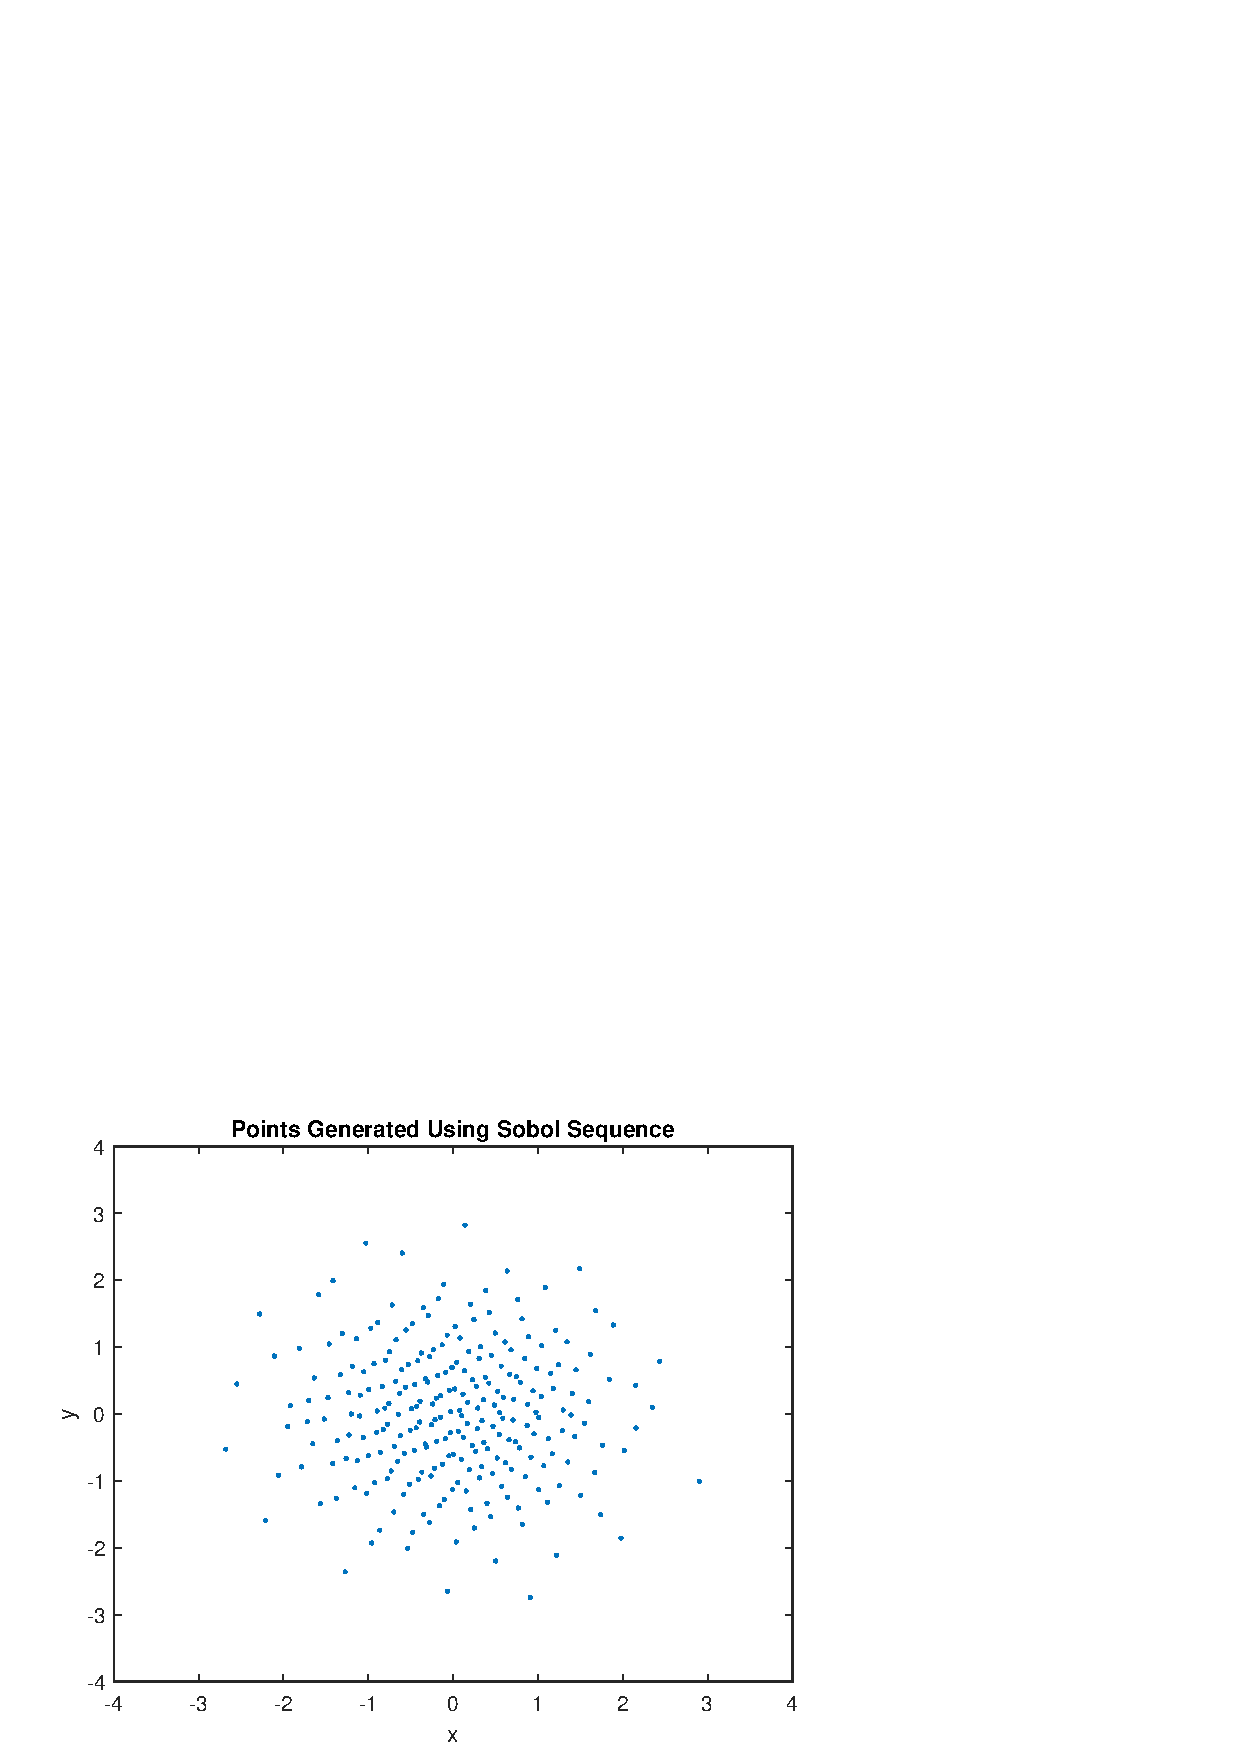
\includegraphics[width=0.7\textwidth]{SobolPoints}
\end{center}
\end{block}

\vspace{.1in}

\begin{block}{\Large \textbf{\blue {Model Problem}}}
\vspace{.1in}
\begin{itemize}
\item Bayesian inference is applied to logistic regression.

\item $t_i \sim \text{Ber} \left(\frac{\exp{\left(\beta_0+\sum_{j=1}^d\beta_j s_{ij}\right)}} {1+\exp \left({{\beta_0+\sum_{j=1}^d\beta_js_{ij}}}\right)}\right), \text{for } i=1, 2, \dots , M$

\vspace{.05in}

\item The prior: standard normal with respect to $\hat{\beta}_j$

\vspace{.05in}

$\pi(\beta)=\frac{\exp{\left({-\frac{1}{2}\beta^T\beta}\right )}}{\sqrt{(2\pi)^{d+1}}}$

\vspace{.05in}

\item Widely used Bayesian inference estimator:

\vspace{.05in}

 $\hat{\beta}_j=\frac{\int_{\mathbb{R}^{d+1}}b_jL(b)\pi(b)db}{\int_{\mathbb{R}^{d+1}}L(b)\pi(b)db} =: \frac{\mu_j}{\mu}, ~for\ j=0, 1, 2,\ldots, d$

\vspace{0.05in} 

where $\hat{\beta}$ are the unknown parameters
\end{itemize}
\end{block}

\end{column}


\begin{column}{.015\linewidth} \end{column} %intercolumn space

\begin{column}{.31\linewidth}

\begin{block}{\Large \textbf{\blue {Choice of Density}}}
\vspace{.1in}
\begin{itemize}
\item The ratio $\frac{\mu_j}{\mu}$ cannot be calculated analytically

\item Thus, we rewrite $\mu$ and $\mu_j$  as such: 

\vspace{.1in}

$\mu=\int_{\Re^{d+1}}L(b)\pi(b)db=\int_{\Re^{d+1}}\frac{L(b)\pi(b)}{\rho(b)}\rho(b)db$,

\vspace{.1in}

where $\rho(b)$ is some density.  Thus, $\frac{\mu_j}{\mu}$ can be estimated by sampling from $\rho(b)$ and applying quasi-Monte Carlo cubature.
\item  We have the following choices for $\rho(b)$:
$\begin{array}{rrcl}
1) & \rho & = & \pi \\
2) & \rho & = & \rho_{\text{MLE}} = \text{Gaussian approximation to the}\\ 
&&&\hspace{4.5cm} \text{likelihood}\\
3) & \rho & \propto & \pi \cdot \rho_{\text{MLE}}
\end{array}$

\end{itemize}
\end{block}

\vspace{0.1in}

\begin{block}{\Large \textbf{\blue {New MATLAB Function}}}
\vspace{.1in}
\begin{itemize}

\item Developed  \alert{function} \mcode{BayesianFunction} that \alert{automatically} estimates the unknown parameters $\hat{\beta}$ using GAIL (Choi Et al, 2015)  

\item User control over various inputs

\end{itemize}
\end{block}

\vspace{0.1in}

\begin{block}{\Large \textbf{\blue {Use Case: Uniform Random s-Data}}}

\vspace{0.1in}    

\lstset{basicstyle=\small} 
\begin{lstlisting} 
% s-Data:100 uniform random values in [-2,6] 
M = 100; %number of s-Data values
s = (6+2)*rand(1,M)-2; %s-Data uniform
dim=2; absTol=0.0005; n=5;
densityChoice = [true true true]; 
%Use all 3 densities
BayesianFunction(M, s, dim, absTol, 
                 densityChoice,n)
\end{lstlisting}    

\begin{center}
\scalebox{0.7}{
\begin{tabular}{ |c|c|c| } 
 \hline
 Density & Runtime (seconds) & Samples Taken \\
 \hline 
 $\rho = \pi$ & 86.088 & 2621440\\
 $\rho = \rho_{\text{MLE}}$ & 2.4954 & 81920\\
 $\rho \propto \pi \cdot \rho_{\text{MLE}}$ & 1.3744 & 40960\\
 \hline
\end{tabular}
}
\end{center}

\begin{center}
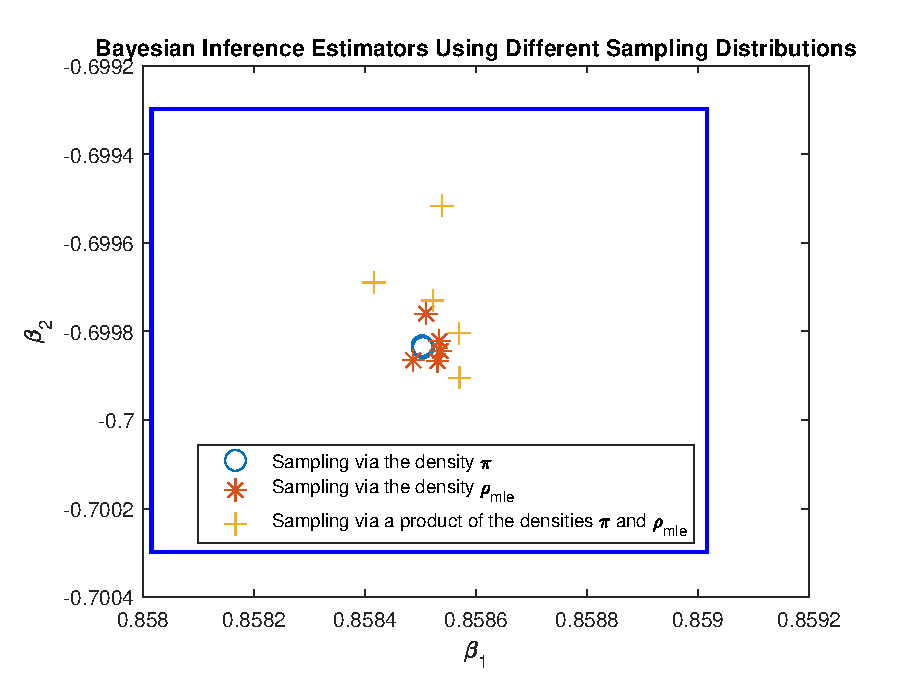
\includegraphics[width=0.7\textwidth]{UniformRandom}
\end{center} 
\end{block}
\end{column}

\begin{column}{.015\linewidth} \end{column} %intercolumn space

\begin{column}{.31\linewidth}
\begin{block}{\Large \textbf{\blue {Use Case: Normal Random s-Data}}}

\vspace{0.1in}    

\lstset{basicstyle=\small} 
\begin{lstlisting} 
% s-Data: 100 normal random values
% with mean 2 and variance 4      
M = 100; %number of s-Data values
u = 2; %mean
sd = 2; %standard deviation
s = sd.*randn(1,M)+u; %s-Data normal
dim=2; absTol=0.0005; n=5;
densityChoice = [true true true];
%Use all 3 densities
BayesianFunction(M, s, dim, absTol, 
                 densityChoice,n)
\end{lstlisting}     

\begin{center}
\scalebox{0.7}{
\begin{tabular}{ |c|c|c| } 
 \hline
 Density & Runtime (seconds) & Samples Taken \\
 \hline 
 $\rho = \pi$ & 13.7314 & 327680\\
 $\rho = \rho_{\text{MLE}}$ & 0.89835 & 20480\\
 $\rho \propto \pi \cdot \rho_{\text{MLE}}$ & 1.4781 & 32768\\
 \hline
\end{tabular}
}
\end{center}

\begin{center}
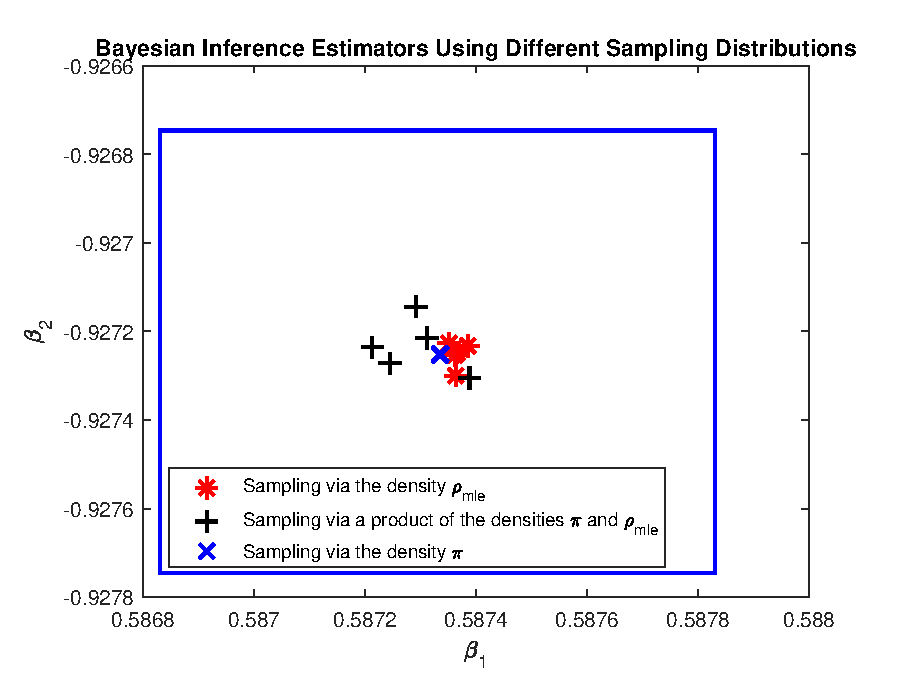
\includegraphics[width=0.7\textwidth]{NormalRandom}
\end{center} 

\end{block}

\bigskip

\begin{block}{\Large \textbf{\blue {Discussion}}}

\vspace{.1in}

\begin{itemize}
\item Add some 

\item Concluding 

\item Remarks here
\end{itemize}

\end{block}

\bigskip

\begin{block}{\Large \textbf{\blue {References}}}

\vspace{.1in}
\begin{itemize}
\item Choi, S.C.T., Ding, Y., Hickernell, F.J., Jiang, L., Jimenez Rugama,
Ll.A., Tong, X., Zhang,Y., Zhou, X. \emph{{GAIL}:
  {G}uaranteed {A}utomatic {I}ntegration {L}ibrary (version 2.1)}, MATLAB
  software, 2015.

\item Hickernell, F.J., Jimenez Rugama, Ll.A., Li, D.
Adaptive Quasi-Monte Carlo Methods for Cubature.

\item Brooks-Bartlett, Jonny. Probability Concepts Explained: Bayesian Inference for Parameter Estimation. Towards Data Science. Retrieved August 5, 2018.
\end{itemize}
\end{block}

\vspace{0.1in}

\begin{block}
{\footnotesize{\black{A special appreciation and thank you to the IIT College of Science for providing the funding behind this research project.}}}
\end{block}

\end{column}
\end{columns}

\end{frame}
\end{document}